\section{أنواع خوارزميات الملاحقة التي تعتمد  التعلم العميق}
يمكن تصنيف ملاحقات التعلم العميق بحسب المرجع
\textLR{\cite{Marvasti}}
 كما يلي:
 \subsection{بنية الشبكة المستخدمة}
 إما أن تكون شبكات
 \textLR{Transformer,GAN,RNN,SNN,CNN}
 أو شبكة مصممة خصيصا لغرض الملاحقة
 \subsubsection{
 	الشبكات العصبونية التلافيفية
 \textLR{CNN Convolutional Neural Networks}}
استخدمت الشبكات التلافيفية في كثير من خوارزميات الملاحقة وذلك لقدرتها على إعطاء تمثيل للغرض بشكل أفضل من الشبكات الأخرى في حال وجود معطيات تدريب كافية،
لكنها غير ملائمة للتدريب أثناء الملاحقة
\textLR{online training}
بسبب التعقيد الحسابي الكبير.
مثل ملاحق 
 \textLR{MDNet \cite{MDNet}}.
 \begin{figure}[h!]
 	\centerline{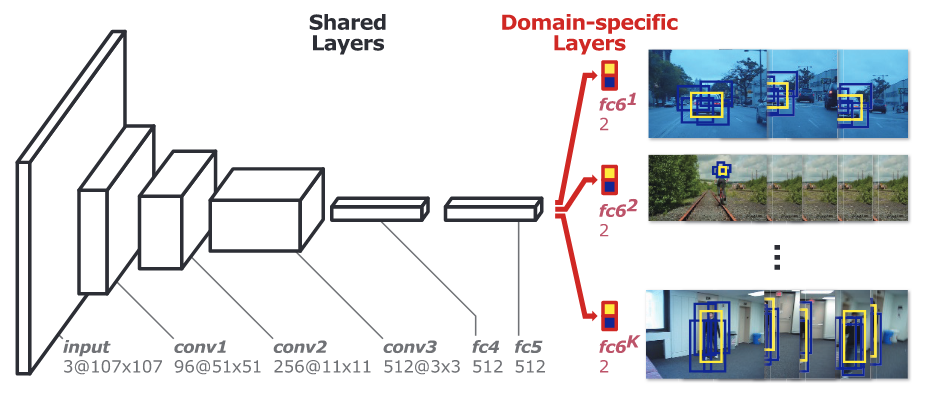
\includegraphics[width=\textwidth]{images/MDNet}}
 	\caption{\textRL{بنية الملاحق}
		\textLR{MDNet} 		 		
 		\textRL{الذي يستخدم شبكات تلافيفية}
 		\textLR{\cite{MDNet}}}	
 \end{figure}
\subsubsection{الشبكات التوأمية 
\textLR{SNN Siamese Neural Networks}}
سميت الشبكات التوأمية بذلك لأنها تتكون من شبكتين متطابقتين في البنية و الأوزان. في معظم تطبيقات الملاحقة يكون دخل الشبكة الأولى هو 
\textLR{template}
الغرض، أما دخل الشبكة الثانية فهو نافذة البحث. انتشر استخدام هذا النوع من الشبكات في خوارزمية الملاحقة بالزمن الحقيقي، لأنها ليست بحاجة إلى تعديل الأوزان أثناء الملاحقة، إذ يكفي تدريب الشبكة بشكل 
\textLR{offline}.
من الممكن أيضاً استخدام أي نوع من الشبكات ضمن الشبكة التوأمية مثل الشبكات التلافيفية كخوارزمية 
\textLR{GOTURN\cite{GOTURN}}
الموضحة في الشكل 
\ref{fig:GOTURN},
أو كمحول 
\textLR{Swin\cite{swintransformer}}
كما في 
\textLR{SwinTrack\cite{swinTrack}}
وهو النموذج الأساسي في بحثنا.
\begin{figure}[h!]
	\centerline{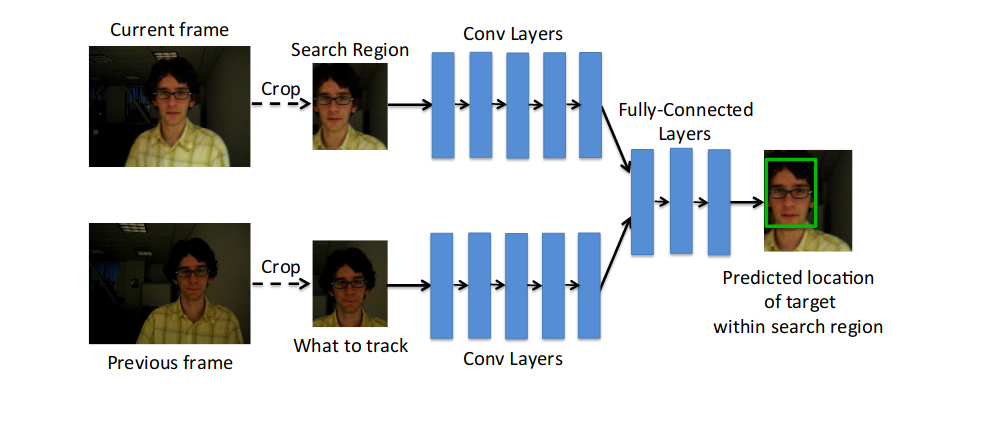
\includegraphics[width=\textwidth]{images/GOTURN}}
	\caption{
		\textRL{بنية الملاحق}
		\textLR{GOTURN}
		\textRL{الذي يستخدم شبكة توأمية مع تلافيفية}
		\textLR{\cite{GOTURN}}}	
	\label{fig:GOTURN}
\end{figure}
\subsubsection{الشبكات العصبونية العودية
\textLR{RNN Recurrent Neural Networks}}
بما أن الملاحقة لاتتعلق فقط بالمعلومات المكانية بل أيضاً بالمعلومات الزمانية، تم استخدام شبكات 
\textLR{RNN}
في مجال الملاحقة ولكن  بشكل محدود، نذكر منها خوارزمية 
\textLR{FPRNet}
\textLR{\cite{Ma18}}

\subsubsection{المحول 
\textLR{Transformer}}
لاقى نموذج المحول نجاحاً كبيراً في مجال معالجة اللغات الطبيعية 
\textLR{\cite{Vaswani17}}،
وبسبب هذا النجاح تم استخدامه في تطبيقات الرؤية الصنعية مثل كشف الأغراض كما في خوارزمية
\textLR{DETR\cite{DETR}}.
 وقد تم استغلاله لأغراض الملاحقة في العامين الأخيرين كما في خوارزميات 
\textLR{STARK\cite{Stark},
TrTr\cite{TrTr} ,
SwinTrack \cite{swinTrack}}.
\subsection{التدريب}
إما أن يكون التدريب 
\textLR{Online}
أو
\textLR{Offline}
 أو كلاهما معاً.
 الكثير من خوارزميات التعلم العميق تستفيد من خرج الشبكات المدربة مسبقاً على مهام مشابهة، والملاحقة مسألة مشابهة لكشف أو تصنيف الصور، لذلك نرى العديد من خوارزميات الملاحقات تستخدم شبكات مثل 
\textLR{ResNet\cite{ResNet},
VGG\cite{VGG}}
كـ
\textLR{backbone}
لاستخلاص السمات من الصور.


يمكن الاستفادة من بعض طبقات هذه الشبكات، أو تعديل بعض أو كل الأوزان بإجراء ضبط نهائي
\textLR{fine tuning}.
\subsubsection{
التدريب بشكل
\textLR{offline}}
معظم ملاحقات التعلم العميق تقوم بعملية التدريب بشكل
\textLR{offline}
وذلك بالاستفادة من مجموعات المعطيات الخاصة بالملاحقة مثل مجموعة المعطيات
\textLR{GOT-10k\cite{got10k},
	 LaSOT\cite{Lasot},
	 TrackingNet\cite{Trackingnet}}
وغيرها.
إذ أن التدريب بشكل  
\textLR{offline}
مناسب لتطبيقات الزمن الحقيقي لأن أوزان النموذج لاتحتاج إلى تعديل أثناء عملية الملاحقة، كما أن ذلك يقلل من انحياز النموذج نحو أغراض معينة 
\textLR{overfitting}
نتيجة التدريب بشكل 
\textLR{online}.
معظم الملاحقات الحديثة يتم تدريبها فقط بشكل 
\textLR{offline}
مثل
\textLR{
STARK\cite{Stark},
SiamRPN++\cite{SiamRPN++},
SwinTrack\cite{swinTrack}}
وغيرها الكثير.
\subsubsection{
التدريب بشكل 
\textLR{Online}
}
من المعروف أن تدريب نماذج التعلم العميق يحتاج زمن طويل وقدرة حسابية عالية، وفي حال عدم توفر عتاد صلب ملائم للتدريب من الممكن اللجوء إلى التدريب بشكل
\textLR{online}
لبعض النماذج، وذلك بتعديل بعض أو كامل أوزان النموذج.
نذكر منها خوارزمية 
\textLR{DeepTrack\cite{DeepTrack},SMART\cite{SMART}}.

\subsubsection{التدريب 
\textLR{online}
و 
\textLR{offline}
معاً}
يمكن جمع طريقتي التدريب السابقتين وذلك بتدريب النموذج بشكل
\textLR{offline}
في البداية
باستخدام مجموعات المعطيات الخاصة بالملاحقة، وبعد ذلك يتم تعديل كامل أو بعض أوزان النموذج أثناء عملية الملاحقة. وذلك كما في خوارزميات 
\textLR{ATOM\cite{ATOM},
	 MDNET\cite{MDNet},
	 DiMP\cite{DIMP},
	 PrDiMP\cite{prDIMP}}.
\subsubsection{}
و كغيرها من نماذج تعلم الآلة فإن خوارزميات الملاحقة التي تعتمد تقنيات التعلم العميق تستخدم تعزيز المعطيات
\textLR{data  augmentation}
 لتقليل الـ
\textLR{ overfitting}،
 وهي طريقة لزيادة حجم مجموعة المعطيات باستخدام بعض التقنيات كاستخدام تحويلات إما في الفضاء الهندسي أو اللوني أو غيرها.
\subsection{غرض الشبكة}
إما أن يكون غرض الشبكة التصنيف 
\textLR{classification}
 أو الـ 
\textLR{regression}
 أو كلاهما معاً.

\subsubsection{التصنيف}
تستخدم الكثير من  الملاحقات أساليب الخوارزميات الأخرى المشابهة لها في  المهام ككشف أو تصنيف الأغراض في الصور وغيرها، ومن هذه الأساليب هي توليد العديد من المناطق المرشَّحة تدعى بـ
\textLR{candidates}
أو بـ
\textLR{proposal bounding boxes}
 المستخلصة من نافذة البحث، ويكون هدف الشبكة هو تصنيف هذه المناطق إما كغرض أو كخلفية. وبالتالي يدرب النموذج وفق هذا المعيار وتستخدم العديد من توابع الخسارة لهذا الغرض مثل 
\textLR{cross-entropy CE,
	focal loss FL\cite{FocalLoss}،
	varifocal loss VL\cite{varifocal}}،
وغيرها، كملاحقات 
\textLR{SiamFC\cite{SiamFC} , DeepTrack\cite{DeepTrack}}.
\subsubsection{
\textLR{Regression}
}
غرض الشبكة في هذه الحالة هو تحديد مكان وأبعاد المستطيل المحيط للغرض بشكل مباشر باستخدام توابع خطأ تعتمد على
\textLR{L1}
 أو
\textLR{L2}،
كما في 
\textLR{GOTURN\cite{GOTURN}}.

\subsubsection{التصنيف والـ
\textLR{regression}
معاً}
 العديد من الملاحقات  قد استخدمت كلتا الطريقتين للتنبؤ بمكان الهدف، إذ يتم توليد العديد من المناطق المرشحة وتحديد المنطقة الأكثر شبهاً بالغرض من خلال شبكة تصنيف، وتحديد أبعاد المستطيل المحيط و زيادة دقة التنبؤ بموقع الغرض من خلال شبكة 
\textLR{regression}،
كما في 
\textLR{MDNet\cite{MDNet}, SwinTrack\cite{swinTrack}, DiMP\cite{DIMP}, SiamRPN++\cite{SiamRPN++}} 
وغيرها.
\subsection{خرج الشبكة}
تبعاً لغرض الشبكة فإن الخرج يمكن أن يكون
\begin{itemize}
	\item خريطة الاستجابة: او ما يدعى بـ 
	\textLR{Confidence}
أو
	\textLR{Response Map}
وهي عبارة عن مصفوفة من القيم ضمن المجال
	$[0,1]$،
وكل قيمة تعبر عن احتمالية وجود الغرض  في الموقع المقابل لها	كما في 
	\textLR{SiamFC\cite{SiamFC}, ATOM\cite{ATOM}, DiMP\cite{DIMP}, SMART\cite{SMART}, PrDiMP\cite{prDIMP}}.
	\item 
	المستطيل المحيط بالغرض: ويمكن أن يعبر عنه بإحداثيات زاويتي المستطيل المتقابلتين، أو بإحداثيات المركز مع أبعاد المستطيل،
	كما في 
	\textLR{GOTURN\cite{GOTURN}, SiamRPN++\cite{SiamRPN++}}
	\item 
	نتيجة التشابه
		 \textLR{similarity score}
		 مثل
		 \textLR{MDNet\cite{MDNet}, DeepTrack \cite{DeepTrack}, SiamRPN++ \cite{SiamRPN++}}
	\item 
	قناع التجزئة
	\textLR{Segmentation Mask}
	مثل خوارزمية 
	\textLR{SiamAttn \cite{SiamAtt}}.
\end{itemize}
هذا فيما يخص أنواع خوارزميات الملاحقة، في الفقرة التالية سنشرح عن نموذج المحول، وعن النماذج السابقة له وكيفية تطور بنيته، وسنشرح عن تابع الانتباه 